\documentclass[oneside,a4paper,14pt]{extarticle} %размер шрифта 14
\usepackage[T2A]{fontenc} 
\usepackage[top=20mm,bottom=20mm,
            left=30mm,right=10mm]{geometry}

\usepackage[utf8]{inputenc} %кодировка текста
\usepackage[russian]{babel} %поддержка русского языка
\usepackage{textcomp} %текстовые символы
\usepackage{indentfirst} %корректировка отступов
\usepackage{graphicx} %работа с изображениям
\usepackage{mwe} % for blindtext and example-image-a in example
\usepackage{wrapfig}
\usepackage{caption}
\usepackage{amsmath}  % для формул и символов
\usepackage{amsfonts}
\usepackage{amsthm}
\usepackage[all]{xy}
\usepackage[breaklinks]{hyperref}
\usepackage{titlesec} 
\usepackage{listings}
\usepackage{minted, fancyvrb}

\setminted{style = rainbow_dash, fontsize = \small}

\titleformat{\section}
{\normalsize\bfseries} 
{\thesection} {1em}{} 
\titleformat{\subsection}
{\normalsize\bfseries}
{\thesubsection} {1em}{} 
\titleformat{\subsubsection}
{\normalsize\bfseries}
{\thesubsubsection} {1em}{} 

\renewcommand\baselinestretch{1.33}\normalsize % межстрочный интервал
\setlength{\parindent}{1.25cm}


\begin{document}
\newpage\thispagestyle{empty}
\begin{center}
	МИНИСТЕРСТВО НАУКИ И ВЫСШЕГО ОБРАЗОВАНИЯ\\
	РОССИЙСКОЙ ФЕДЕРАЦИИ\\
	ФЕДЕРАЛЬНОЕ ГОСУДАРСТВЕННОЕ БЮДЖЕТНОЕ\\
	ОБРАЗОВАТЕЛЬНОЕ
	УЧРЕЖДЕНИЕ ВЫСШЕГО ОБРАЗОВАНИЯ\\
	«ВЯТСКИЙ ГОСУДАРСТВЕННЫЙ УНИВЕРСИТЕТ»\\
	Институт математики и информационных систем\\
	Факультет автоматики и вычислительной техники\\
	Кафедра электронных вычислительных машин
\end{center}
\vspace{30mm}

\begin{center}
	Отчёт по лабораторной работе №1\\
	по дисциплине\\
	<<Управление данными>>\\
	<<Основы DDL-запросов в PostgreSQL .>>\\
\end{center}
\vspace{40mm}

\noindent
\begin{tabular}{l r}

	Выполнил студент гр. ИВТб-2303-06-00
	\hspace{10mm} \rule[-1mm]{20mm}{0.15mm}\,/Перевозчиков Д.А./ \\ \\


	Проверил
	\hspace{57mm}
	\rule[-1mm]{20mm}{0.15mm}\,/Клюкин В. Л./
\end{tabular}

\vfill
\begin{center}
	Киров\\
	2026
\end{center}


\newpage\thispagestyle{empty}

\section{Цели лабораторной работы:}
\begin{itemize}
	\item познакомиться со схемами, пользователями и ролями в PosgreSQL;
	\item познакомиться с типами данных в PostgreSQL; 
	\item освоить основные варианты DDL-запросов в PostgreSQL; 
	\item закрепить знания по проектированию структуры реляционной БД; 
	\item создать рабочий материал для следующих лабораторных работ. 
\end{itemize}


\section{Задание:}
\begin{enumerate}
	\item Разработать структуру базы данных на любую выбранную тему. \\
	      {Структура должна отвечать следующим условиям: }
	      \begin{itemize}
	      	\item  должно быть не меньше пяти таблиц;
	       	\item  хотя бы одна таблица должна содержать  колонку с числовыми данными;
	      	\item  структура БД не должна быть связь много-ко-многим; \\
	      \end{itemize}

	\item Создать нового пользователя и пустую БД. Подключиться к созданной БД.  \\
	
	\item Написать и выполнить SQL-скрипт, создающий таблицы согласно разработанной структуре БД. Созданный в п.2 пользователь должен иметь все права на созданные объекты. В этом же скрипте должны создаваться нужные ограничения и индексы:   \\
	
	\begin{itemize}
		\item обязательно должны быть созданы внешние ключи для поддержания ссылочной целостности; 
		\item желательно должны быть проставлены ограничения и уникальные индексы для поддержания консистентности данных (например, если в таблице есть столбец с температурой воздуха за окном, стоит ограничить возможный промежуток значений); 
		\item желательно должны быть проставлены индексы для производительности там, где они могут помочь (из расчета, что созданная БД будет хранить достаточно большое количество данных;
	\end{itemize}


\end{enumerate}


\newpage
\section{Решение:}
\subsection[short]{Задание 1.}
Для выполнения задания смоделируем такие условия:
Необходимо спроектировать базу данных для хранения информации о доступных ресурсах гоночного клуба. Проектируемая система должна выполнять следующие действия: 
\begin{itemize}
\item Редактировать автопарк - набор гоночных автомобилей, гоночный автомобиль можно добавить, редактировать информацию, отправить в утилизацию. Автомобилем в утилизации клиенты воспользоваться не могут.  
\item Гоночный автомобиль состоит из заголовка, фото, описания, кол-ва лошадиных сил, года выпуска, цвета, наименования подвески.  
\item Редактировать тренерский состав - добавлять, удалять, редактировать информацию о тренере.  
\item Информация о тренере включает в себя ФИО, года рождения, номер счёта в банке для начисления заработной платы, фото тренера, список достижений тренера, список автомобилей, на которых тренер может тренировать. А также любимый автомобиль тренера.  
\item Список достижений тренера состоит из элементов, каждый из которых включает в себя наименование соревнования, дату проведения соревнования и занятое место.

\end{itemize} 

Учитывая все вышеперечисленные требования, разработаем схему базы данных гоночного клуба.


ER-диаграмма для задания 1 представлена на Рисунке 1.\\
Исходный код представлен в Приложении А1. %\ тут мы код не вставляем!!!
\begin{flushleft}
\begin{figure}[h!]
	\centering
	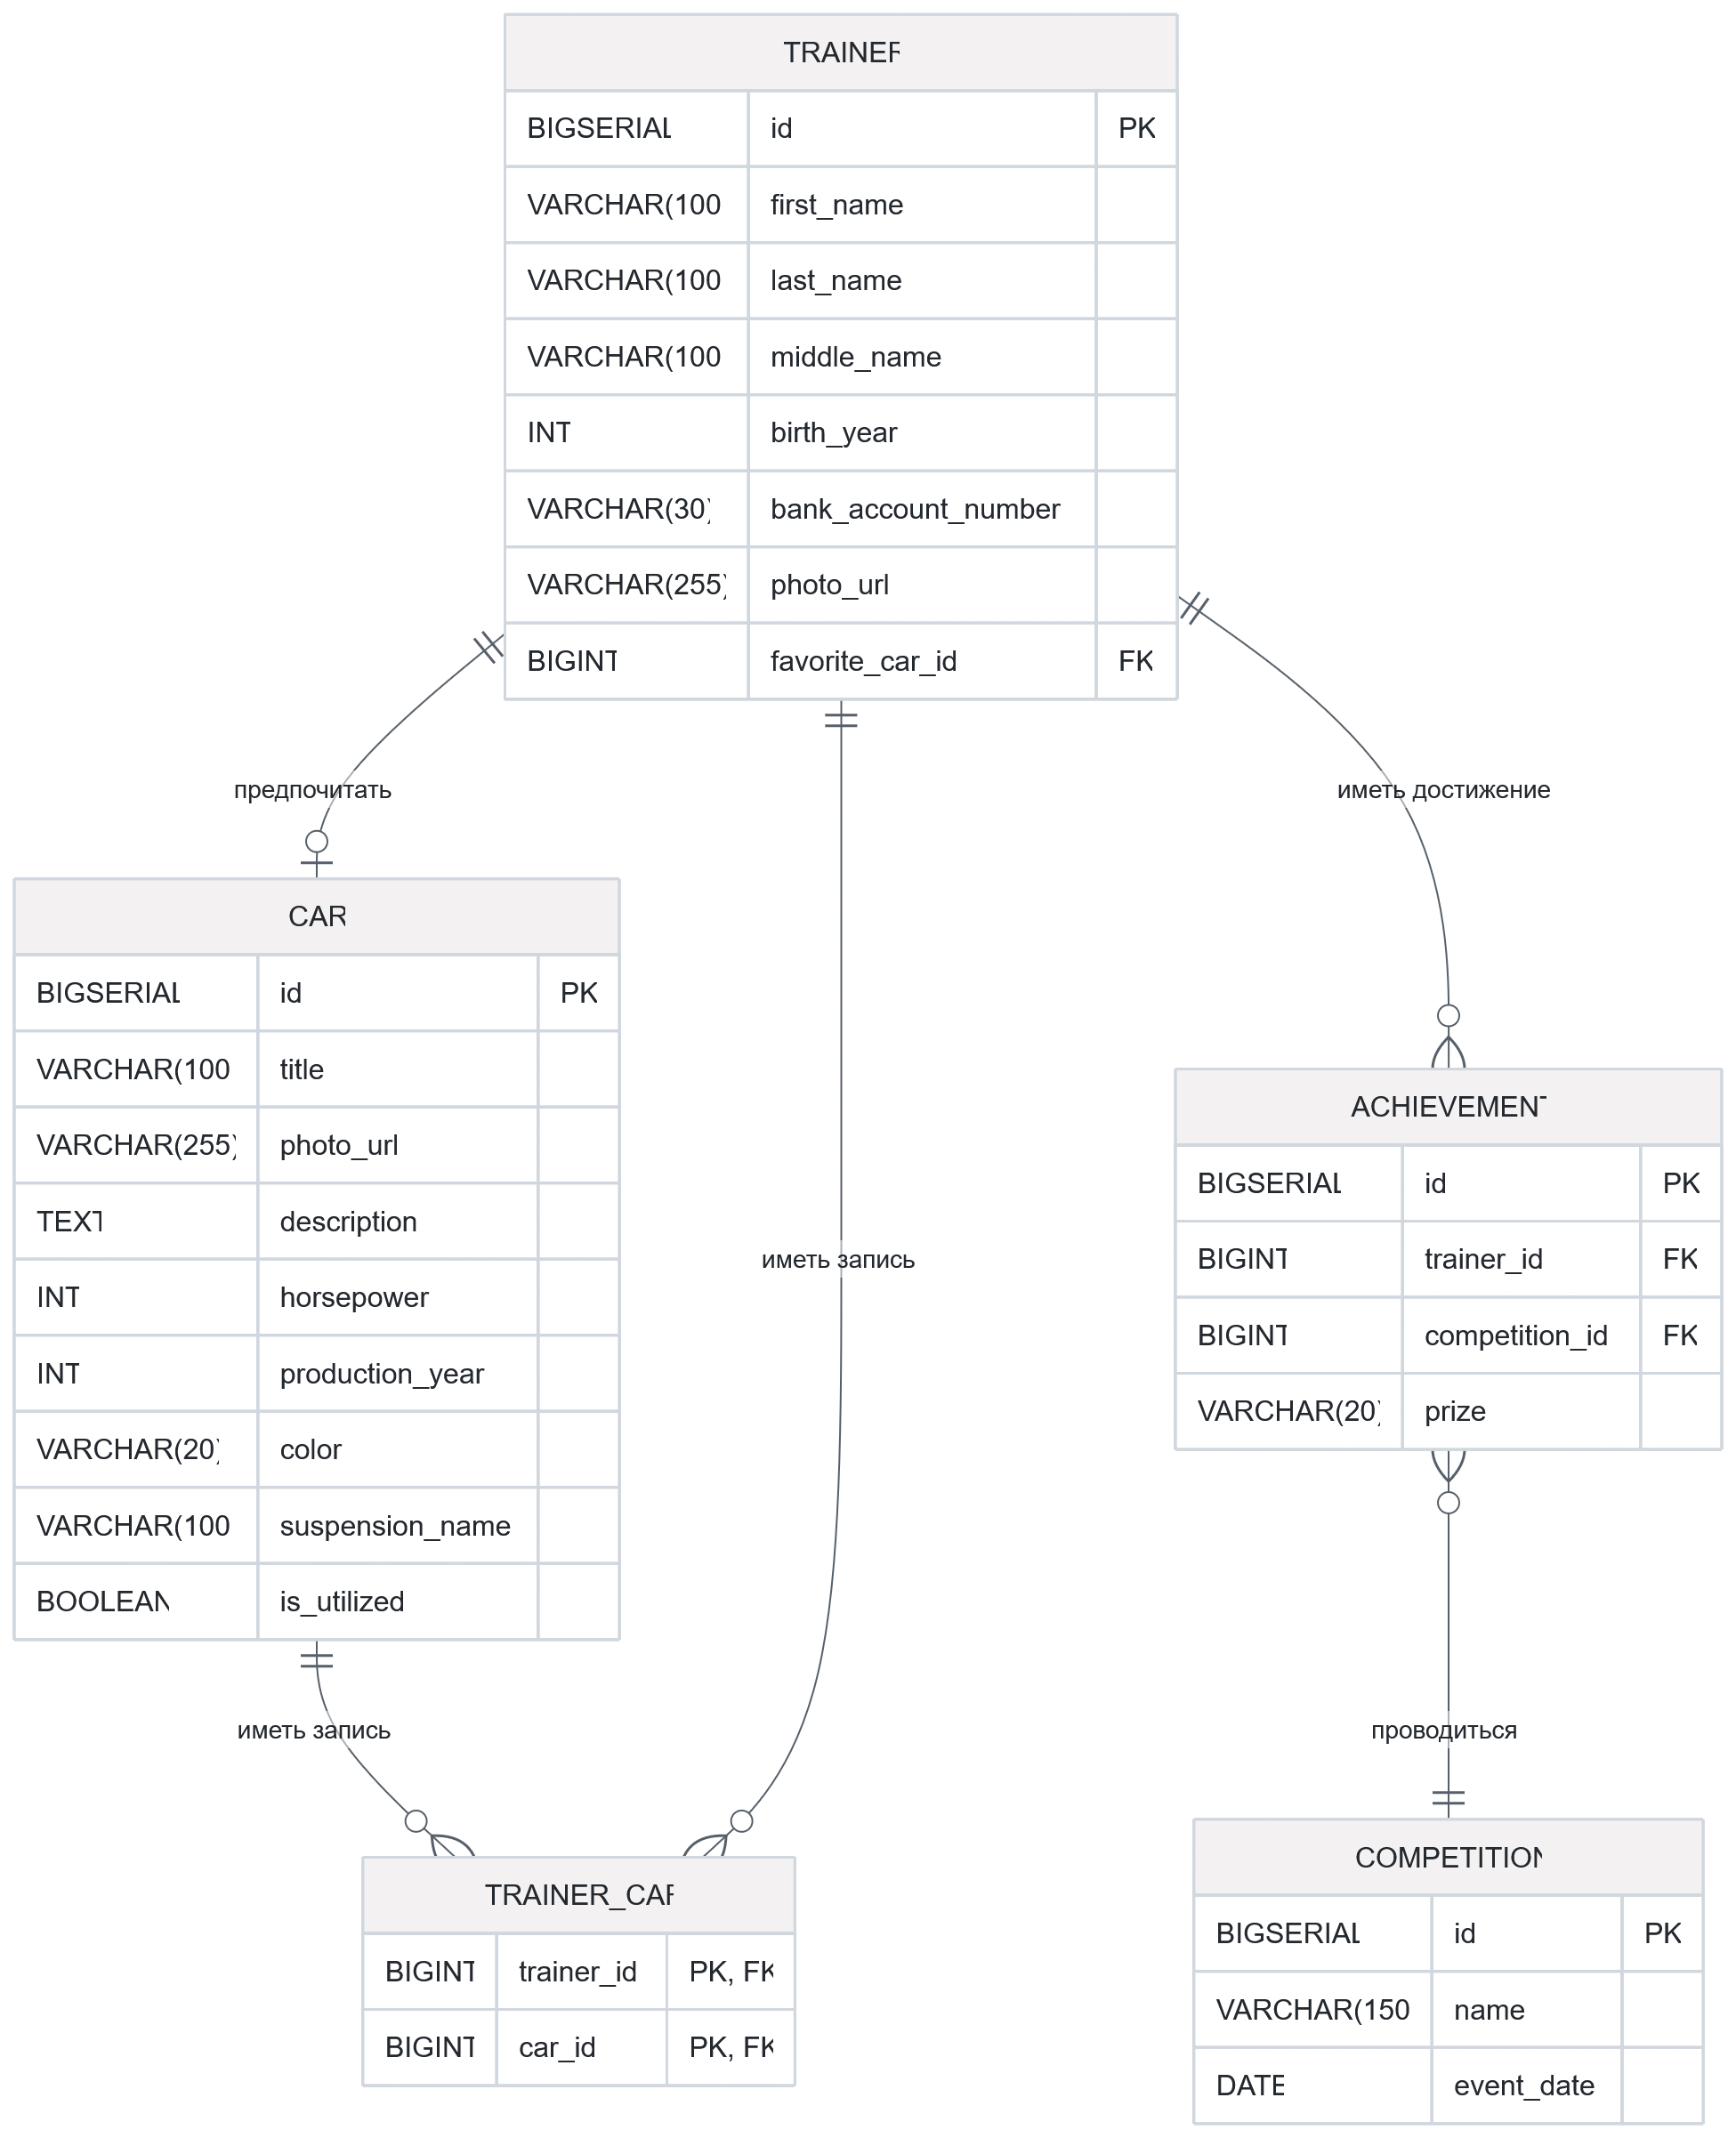
\includegraphics[width=0.85\textwidth]{images/er.png} 
	%\ если у вас не влезает картинка уменьшите параметр width=
	\caption*{Рисунок 1 - ER диаграмма задания 1}
\end{figure}
\end{flushleft}


\newpage
\subsection[short]{Задание 2.}
С использованием консольной утилиты \textbf{psql} был создан пользователь базы данных roiten. От его имени была создана база для решения задачи от автоклуба. 
\begin{flushleft}
\begin{figure}[h!]
	\centering
	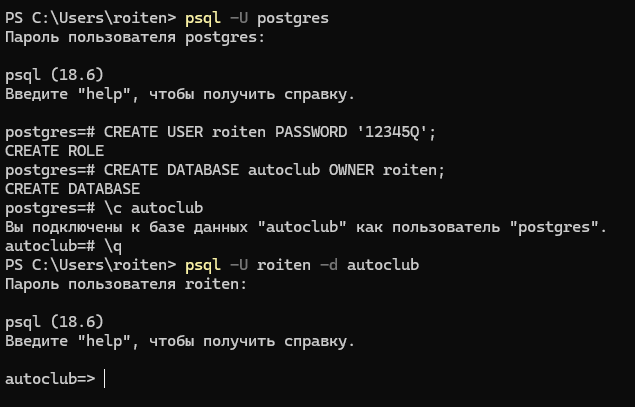
\includegraphics[width=0.85\textwidth]{images/create_db.png} 
	\caption*{Рисунок 2 - Создание пользователя и базы данных.}
\end{figure}
\end{flushleft}


\newpage
\subsection[short]{Задание 3.}
В соответствии с разработанной структурой базы данных были написаны SQL-запросы, создающие все таблицы, внешние ключи, ограничения и индексы. Скрипт выполнен от имени пользователя, созданного в п.2. Полный текст SQL-скрипта со всеми ограничениями и индексами приведён в Приложении А1.


\section*{Вывод:}
В ходе выполнения лабораторной работы были освоены схемы, пользователи и роли в PostgreSQL, типы данных, основные варианты DDL-запросов, а также закреплены знания по проектированию структуры реляционной БД. Создан рабочий материал для следующих лабораторных работ.

\newpage
\begin{flushright} \bf Приложения \end{flushright}
\section*{Приложение A1}
Исходный код запросов для задания 3:
\inputminted{sql}{../autoclub.sql} 
\newpage

\end{document}